\section{ART Model}
\label{sec:model}

\subsection{Architecture}
\label{sec:architecture}
The architecture of ART is shown in Fig.\ref{fig:architecture} . As we can see, the input of  ART consists of two types of features, including content features and social features. Then, all features will be embedded and be sent to filters or classifiers.  Some components such as textCNN or Dense use word-to-vector embeddings and the other components use their own embedding methods. Next, each trained component will make its prediction respectively. Finally, we add the predictable results of all components and give the final prediction. 

\begin{figure}[tbp]
	\hspace{0ex}
	\vspace{0ex}
	\centering
	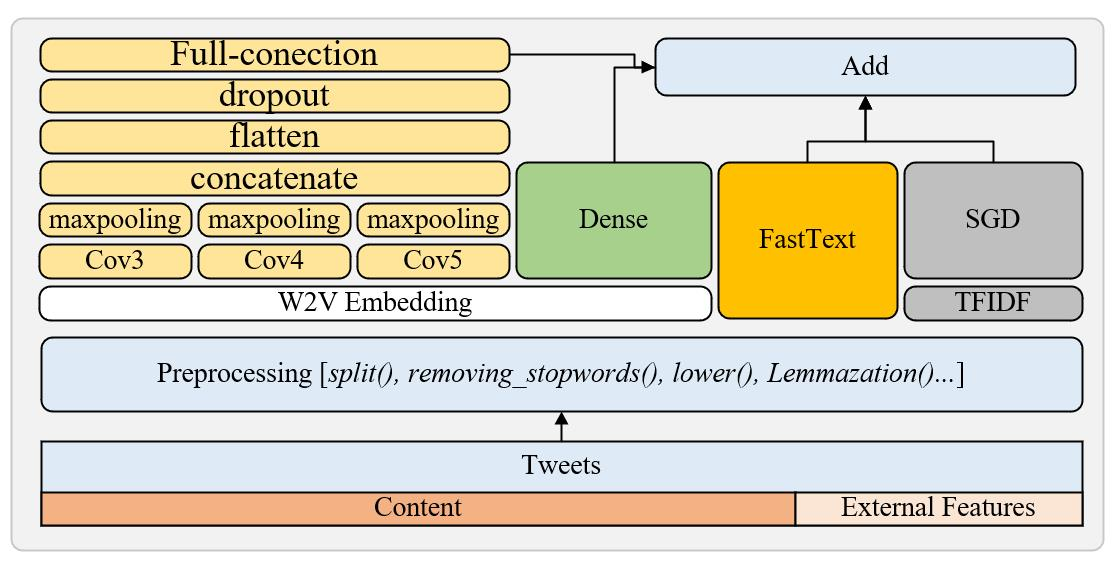
\includegraphics[width = \textwidth]{fig/architecture}
	\caption{Architecture of ART}
	\label{fig:architecture}
\end{figure}

\subsection{Preprocessing and Embedding}
Content is the text of the tweet, which is the most important feature for the rumor tracking task. The text of the tweet is short, which is restricted within 140 words. Usually, the spelling in tweets is causal with symbols mixed in it. Consequently, before input them into the model, we will conduct prepossessing firstly. The prepossessing in NLP is roughly immobilized, we only need to make some minor adjustments. In this work, we adopt splitting on tweets, then removing the punctuation and special characters. Next, we turn all characters into lowercase. Finally, we adopt lemmatization on all words.
 
High-quality embedding of text is a key factor for NLP tasks. Generally speaking, we have three embedding strategies: pre-trained embedding, trained embedding on the current dataset, and random embedding. Pre-trained embedding is trained on a corpus with very big scales, and some of the famous ones are GloVe \cite{pennington2014glove}, Google News embedding\cite{DBLP:journals/corr/abs-1301-3781}. It is common practice to train embedding on the current dataset, and we also do this in PHEME and RumorEval dataset. The last way is using random embedding, which assigns each word with a unique embedding randomly. In this work, we try all three embedding strategies and the detailed performance will be introduced in section \ref{sec:experiment}. By comparing them, we finally choose random embedding as the strategy in ART.

\subsection{Components for Content Features}
After embedding, we send content features to different types of deep learning models. As shown in Fig.~\ref{fig:architecture}, we add TextCNN, SGD, and FastText to dispose of the content feature. These three components are trained respectively until getting convergence. When predicting, each component outputs an m-dimensional vector after the softmax layer. Each dimension suggests the probability that the content belongs to this classification.

\subsection{Components for Social Features}
Despite some content features, the tweets contains plenty of social features, including . As introduced in section \ref{sec:problem}, we should not get any information about tweet's branch or threads in advance. Consequently, we omit some features that contains external branch information. Finally, we choose "screen name" and "hashtag" as the social features in ART. 

\subsection{Details of Aggregation}
With all components trained, we aggregate them and give the final prediction on rumor tracking task. Generally, there are two common used aggregation methods: joint training and respective training. Joint training means all models has one shared optimization function, and all parameters are updated together. Respective training means we train each component respectively. When predicting, 